\subsection{Hardware Implementation}
This section details the hardware implementation for Pookie. Overall, the design consists of a robotic shell housing an array of electronic components including the microprocessor, motors, sensors, and so on. A fully functional hardware implementation was not within the scope for this semester, which focused on a basic software proof of concept, and physical design.


\subsubsection{Initial Design}
\begin{enumerate}

    \item\textbf{Outer Shell Design}
    
    In the initial phase, a preliminary design is developed for the outer shell. The design is inspired by Rilakkuma, a well-known Japanese character created by San-X in 2003. Rilakkuma is recognized for its comforting and cute aesthetic, which represents relaxation and embodies the essence of kawaii culture. Its rounded features and laid-back attitude have made it a popular symbol of comfort and appeal \cite{hinka_rilakkuma_history}.
    
    \begin{figure}[ht]
        \centering
        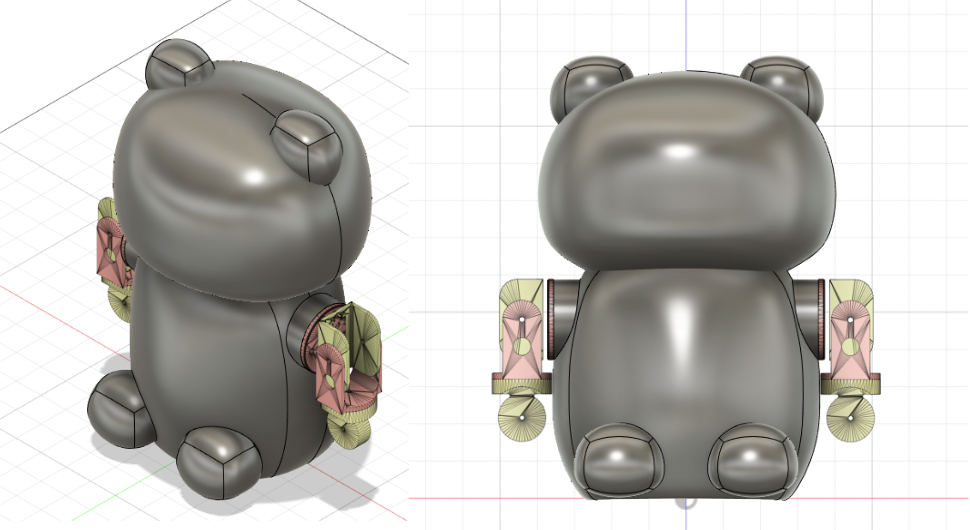
\includegraphics[width=0.6\textwidth]{init-outer.png}
        \caption{Initial Outer Shell Design of Pookie}
        \label{fig:init-outer}
    \end{figure}

    \item\textbf{Inner Shell Mechanism Design}

    The arms are designed to move along the x-axis revolute joint and are powered by CS002 20 Kg servo motors.
    \begin{figure}[ht]
        \centering
        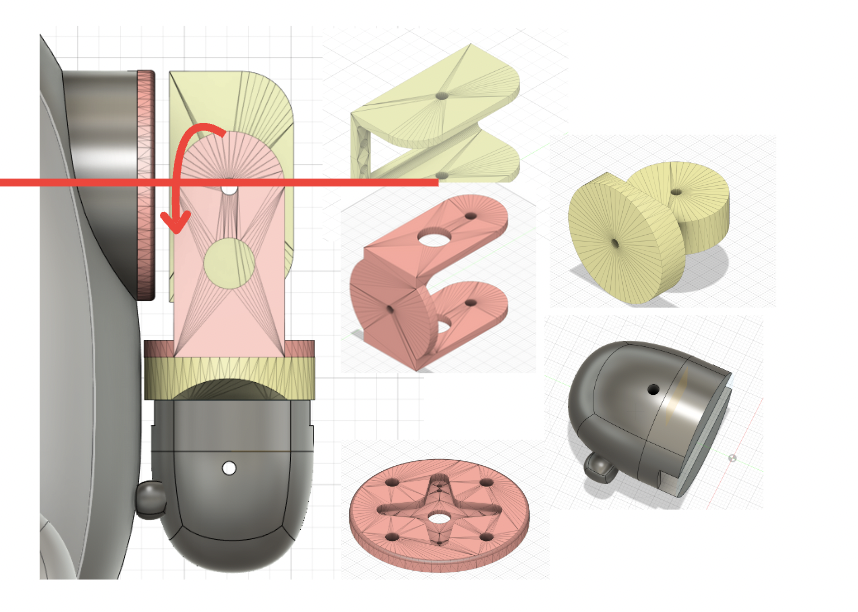
\includegraphics[width=0.6\textwidth]{inner-arm.png}
        \caption{Initial Arm Mechanism of Pookie}
        \label{fig:inner-arm}
    \end{figure}
    
\end{enumerate}
\newpage
\subsubsection{Revised Design}
The revised hardware design of the Pookie robot focuses on anthropomorphic aesthetics, user-centric functionality, seamless mechanical integration, changes in the arm movement axis, and a more compact size.

\begin{figure}[ht]
    \centering
    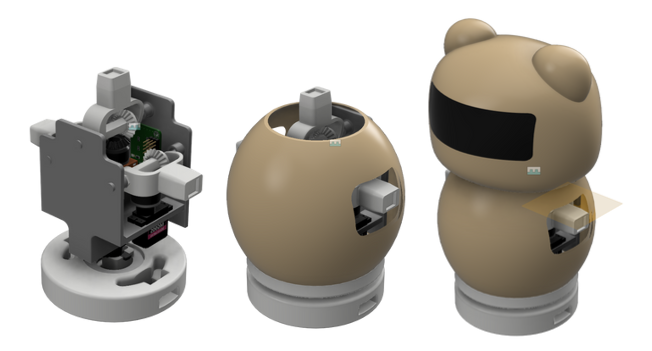
\includegraphics[width=0.8\textwidth]{revised.png}
    \caption{Revised Design of Pookie}
    \label{fig:revised}
\end{figure}

\begin{enumerate}
    \item\textbf{Outer Shell Design}

    The outer shell of Pookie is designed to enclose all internal components in a compact form. It consists of two main sections: the body and the head. The body houses the internal systems, while the head contains an LED screen for displaying the robot's eyes and serves as the mounting point for the head movement mechanism.

\begin{figure}[!ht]
    \centering
    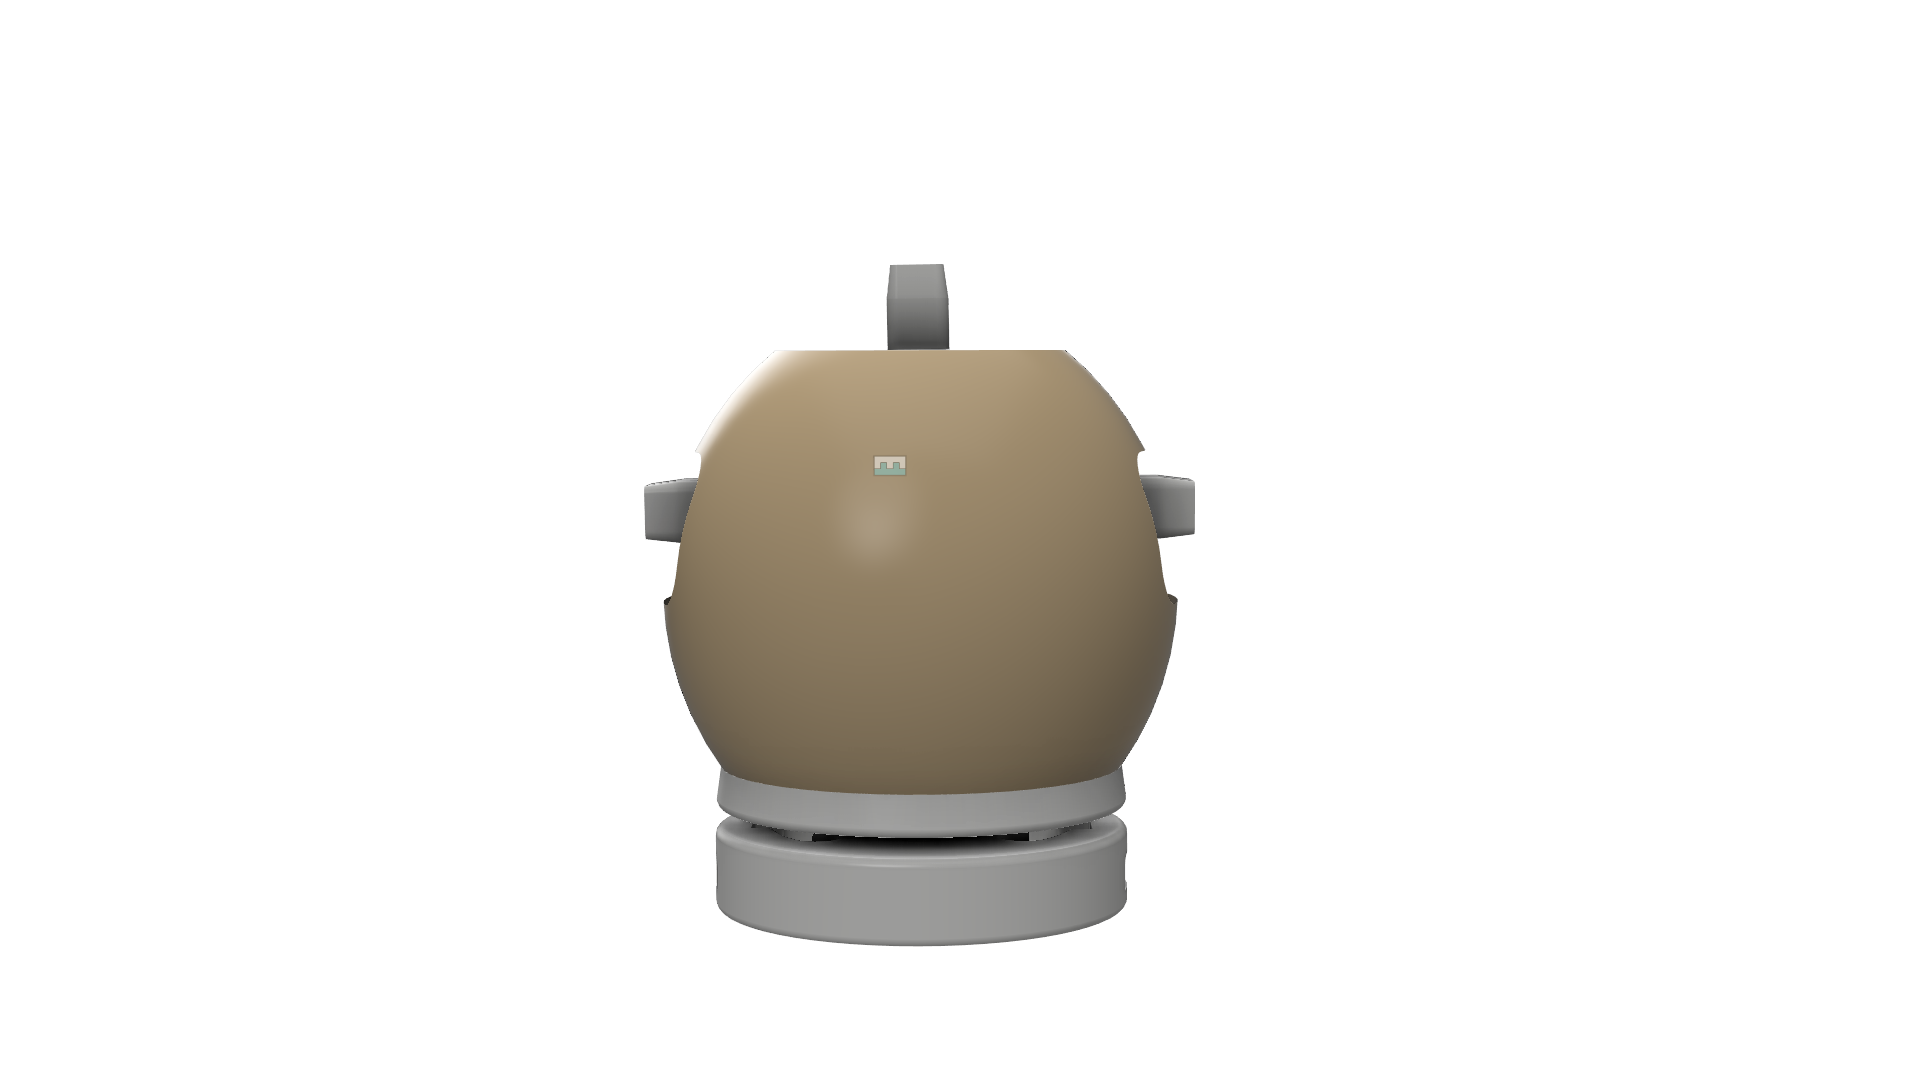
\includegraphics[width=0.8\textwidth]{new_outer.png}
    \caption{Revised Outer Shell Body of Pookie}
    \label{fig:revised_outer}
\end{figure}

\begin{figure}[!ht]
    \centering
    
\includegraphics[width=0.5\textwidth]{new_head.png}
    \caption{Revised Outer Shell Head of Pookie}
    \label{fig:revised_head}
\end{figure}

\newpage
\item\textbf{Inner Shell Mechanism Design}

The movement mechanisms in Pookie include systems for the head, arms, and base. Each actuator is represented as a cylinder, indicating rotational motion driven by MG90s servo motors. The motion occurs along defined axes, with the z-axis primarily supporting rotational movements. 

\begin{figure}[!htb]
    \centering
    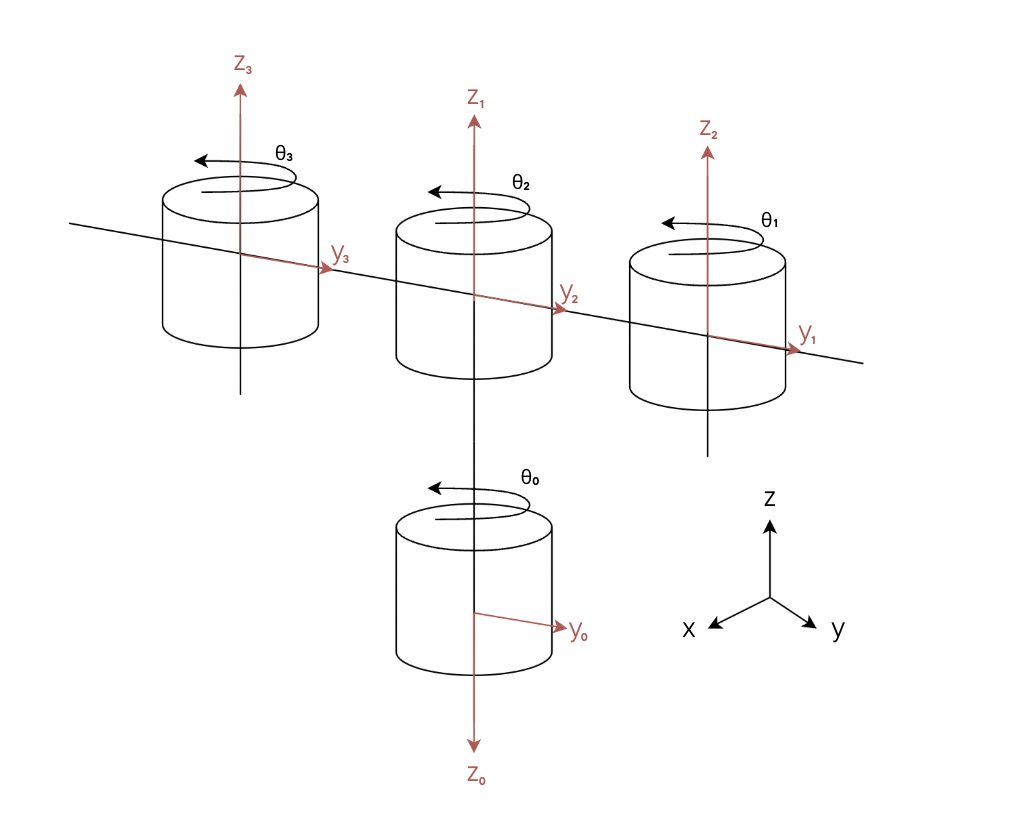
\includegraphics[width=0.7\textwidth]{motion.png}
    \caption{Motion Axes for Pookie's Movement Mechanisms}
    \label{fig:motion}
\end{figure}

Both the head and arm movements use a bevel gear mechanism with a 1:1 transmission powered by MG90s servo motors. This system provides a single degree of freedom along the \textbf{y-axis} revolute joint. A magnet slot at the tip allows easy attachment to the outer shell head, simplifying assembly and maintenance.

\newpage
\begin{figure} [!htb]
    \centering
    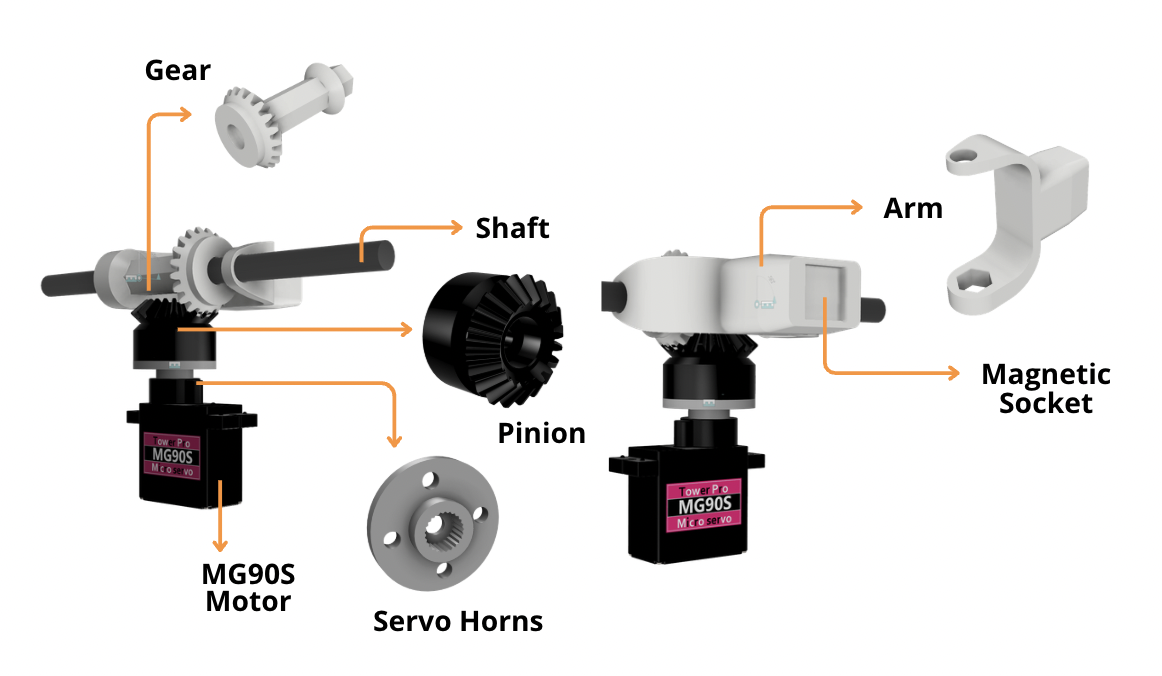
\includegraphics[width=0.7\textwidth]{gear_diagram.png}
    \caption{Components of the Head and Arm Mechanisms}
    \label{fig:components_head_arm}
\end{figure}

The bevel gear mechanism transfers motion from the servo motor to the movement axis efficiently. With a 1:1 transmission ratio, the angular velocity (\(\omega\)) of the driving gear is equal to that of the driven gear. This relationship is expressed as:

\[
\omega_{\text{output}} = \omega_{\text{input}}
\]

where \(\omega_{\text{input}}\) is the angular velocity of the motor, and \(\omega_{\text{output}}\) is the angular velocity of the output gear. Similarly, the angular acceleration (\(\alpha\)) remains unchanged during transmission:

\[
\alpha_{\text{output}} = \alpha_{\text{input}}
\]

This design ensures that the servo motor’s precise control over movement translates directly to the head and arm mechanisms. The torque transmitted by the system is given by:

\[
\tau_{\text{output}} = \tau_{\text{input}}
\]

where \(\tau_{\text{input}}\) is the torque generated by the servo motor. The selection of a 1:1 transmission ratio supports direct coupling, allowing for seamless motion transmission without the need for additional adjustments or gear reduction.

For the base rotation, a bearing-supported system allows full 360-degree rotation along the z-axis. This system incorporates a low-friction bearing assembly, ensuring smooth and precise rotational motion.

\begin{figure}[!htb]
    \centering
    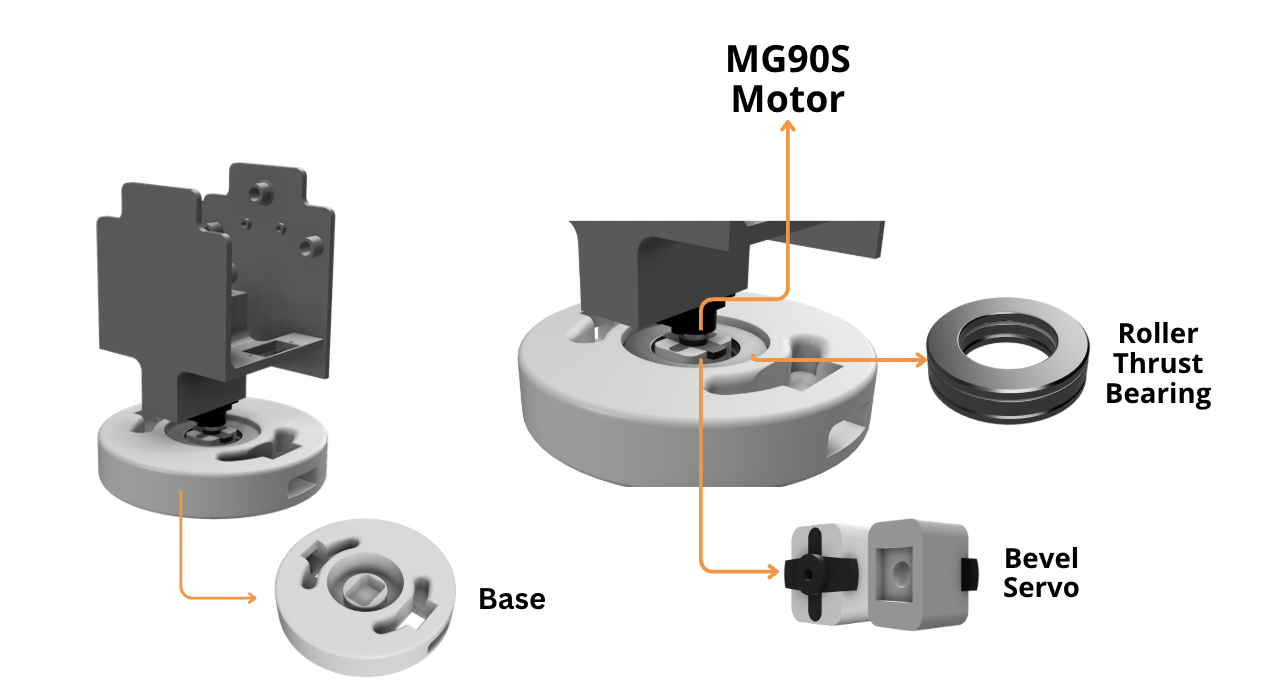
\includegraphics[width=0.7\textwidth]{new_base.png}
    \caption{Components of the Base Mechanism}
    \label{fig:base_comp}
\end{figure}

An armor has been designed to house and support the head, arm, and base rotation mechanisms. It includes compartments for the servo motor and the PWM servo motor driver, as well as openings to facilitate wiring integration. This armor ensures structural integrity and maintains the functionality of all movement mechanisms within Pookie’s compact design.

\begin{figure}[!htb]
    \centering
    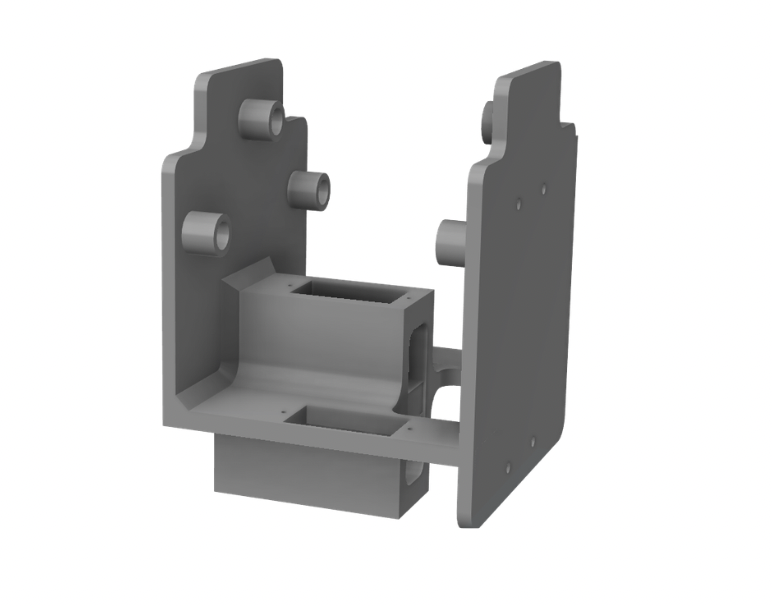
\includegraphics[width=0.7\textwidth]{new_armor.png}
    \caption{Internal Armor Design of Pookie}
    \label{fig:new_armor}
\end{figure}


\end{enumerate}

